%  Beamer slide example.

\documentclass[9pt]{beamer}
\usepackage[utf8]{inputenc}
\usetheme{inria}
\usepackage{helvet}
\usepackage{graphicx}
\usepackage{nameref}

\usepackage{tikz}
\usetikzlibrary{arrows,shapes,positioning,calc,shadows,trees}
\tikzset{
  mstep1/.style = {basic, rounded corners=2pt, thin, align=center, fill=orange!70,text width=1.5cm},
  mstep2/.style = {basic, rounded corners=2pt, thin, align=center, fill=green!30,text width=1.5cm},
  basic/.style  = {draw, text width=2cm, drop shadow, font=\sffamily, rectangle},
  root/.style   = {basic, rounded corners=2pt, thin, align=center,
                   fill=green!30},
  level 2/.style = {basic, rounded corners=6pt, thin,align=center, fill=green!60,
                   text width=8em},
  level 3/.style = {basic, thin, align=left, fill=pink!60, text width=6.5em}
}
\tikzstyle{every picture}+=[remember picture]
\tikzstyle{na} = [baseline=-.5ex]


\def\aboxl[#1,#2,#3,#4,#5]#6{%
  \node[draw, cylinder, alias=cyl, shape border rotate=90, aspect=#3, %
  minimum height=#1, minimum width=#2, outer sep=-0.5\pgflinewidth, %
  color=orange!40!black, left color=orange!70, right color=orange!80, middle
  color=white] (#4) at #5 {};%
  \node at #5 {#6};%
  \fill [orange!30] let \p1 = ($(cyl.before top)!0.5!(cyl.after top)$), \p2 =
  (cyl.top), \p3 = (cyl.before top), \n1={veclen(\x3-\x1,\y3-\y1)},
  \n2={veclen(\x2-\x1,\y2-\y1)} in (\p1) ellipse (\n1 and \n2); }

\author{Maurice Brémond \and Gaëtan Harter}

\title[Intégration continue]{L'Intégration Continue}
% \subtitle{Dans un contexte de développement Inria}
\subtitle{Présentation IJD}

% Automatically insert a "new section" page at each section.
\AtBeginSection[]{
  \begin{frame}[plain]
    \partpage
  \end{frame}
}
% \inriaswitchcolors COLOR
%
% Where COLOR is one of red, blue, orange, darkblue, violet,
% pastelgreen, grey, or green.
\newcommand{\inriaswitchcolors}[1]{%
  \pgfaliasimage{figfootline}{figfootline-#1}% !!!
  \pgfaliasimage{figbackground}{figbackground-#1}% !!!
  \pgfaliasimage{figbackground}{figbackground-#1}% !!!
}

% frame with toc for current subsection
\newcommand{\tocsubsection}{
  \begin{frame}
    \tableofcontents[
      currentsubsection,
      sectionstyle=show/shaded,
      subsectionstyle=show/shaded,
      subsubsectionstyle=show/show/shaded
    ]
  \end{frame}
}
% starting the document
% *********************
\begin{document}

% titlepage
% ---------
\begin{frame}[plain]
  \titlepage
\end{frame}
% table of contents
% -----------------
\begin{frame}{\textcolor{inriaGrey}{Table des matières}}
  \tableofcontents
\end{frame}



% Introduction
% ************

\inriaswitchcolors{red}
\section{Quid de l'intégration continue}

\subsection{Qu'est-ce que c'est}
\begin{frame}{}
\begin{block}{Intégration}
  \begin{itemize}
  \item mise en oeuvre de la chaine de test et de production d'un logiciel
  \end{itemize}
\begin{tikzpicture}
  \node[] (developer1) {
\includegraphics[width=.04\textwidth] {images/Laptop-icon.png}};
  \node[below=.001cm of developer1] (developer2) {
\includegraphics[width=.04\textwidth] {images/Laptop-icon.png}};
  \node[below=.001cm of developer2] (developer3) {
\includegraphics[width=.04\textwidth] {images/Laptop-icon.png}};
  \node[right=1.3cm of developer2] (code_repo_db) {};
  \node[above=.4cm of code_repo_db] (code_repo_db_north) {};
  \node[left=.2cm of code_repo_db] (code_repo_db_west) {};
  \node[below=.1cm of code_repo_db] (code_repo_db_south) {};
  \node[below=.9cm of code_repo_db,mstep1] (code_repo) {gestion de versions};
  \aboxl[25,20,1.6,a1,(code_repo_db)] {};
  \node[right=.6cm of code_repo,mstep2] (build) {fabrication};
  \node[above=.4cm of build] (nux) {
\includegraphics[width=.04\textwidth] {images/Linux-icon.png}};
  \node[above=.001cm of nux] (windows) {
\includegraphics[width=.04\textwidth] {images/Windows-icon.png}};
  \node[above=.001cm of windows] (freebsd) {
\includegraphics[width=.04\textwidth] {images/Apps-freebsd-icon.png}};
  \node[right=.6cm of build,mstep2] (tests) {tests};
  \node[above=.4cm of tests] (test_ok1) {
\includegraphics[width=.02\textwidth] {images/accept-icon.png}};
  \node[above=.001cm of test_ok1] (test_ok2) {
\includegraphics[width=.02\textwidth] {images/accept-icon.png}};
  \node[above=.001cm of test_ok2] (test_bad1) {
\includegraphics[width=.02\textwidth] {images/delete-icon.png}};
  \node[above=.001cm of test_bad1] (test_ok4) {
\includegraphics[width=.02\textwidth] {images/accept-icon.png}};
  \node[right=.001cm of test_ok1] (test_bad1) {
\includegraphics[width=.02\textwidth] {images/delete-icon.png}};
  \node[right=.001cm of test_ok2] (test_ok3) {
\includegraphics[width=.02\textwidth] {images/accept-icon.png}};
  \node[right=.6cm of tests,mstep2] (install) {installation paquetage};
  \node[above=.4cm of install] (package) {
\includegraphics[width=.06\textwidth] {images/System-Package-icon.png}};
  \path[<->, thick, color=blue] (developer1) edge [bend left] (code_repo_db_north);
  \path[<->, thick, color=blue] (developer2) edge [] (code_repo_db_west);
  \path[<->, thick, color=blue] (developer3) edge [bend right] (code_repo_db_south);
  \path[->, thick, color=gray,dotted] (code_repo.east) edge [] (build.west);
  \path[->, thick, color=gray,dotted] (build) edge [] (tests);
  \path[->, thick, color=gray,dotted] (tests) edge [] (install);
\end{tikzpicture}
\end{block}
\begin{block}{en continu}
\begin{itemize}
\item à chaque nouvelle version pour les tests rapides
\item régulièrement : chaque nuit, chaque semaine pour les tests longs.
\end{itemize}
\end{block}
\begin{block}{Pourquoi ?}
  \begin{itemize}
  \item réduire le coût du ``merge''
  \item éviter au plus tôt les régressions
  \item cf extrem programming
  \end{itemize}
\end{block}
\end{frame}

\begin{frame}{La fabrication}
\begin{block}{problématiques}
  \begin{itemize}
  \item quel compilateur, quels arguments
  \item dépendances entre fichiers sources
  \item éditions de liens avec les librairies externes
  \item \dots
  \end{itemize}
\end{block}
\begin{block}{des moteurs de production}
  \begin{itemize}
  \item make
  \item autotools
  \item cmake
  \item scons
  \item qmake
  \item \dots
  \end{itemize}
\end{block}
\end{frame}

\begin{frame}{Le test}
\begin{block}{}
  \begin{itemize}
  \item analyse statique    : pep8, pylint, clang static analyzer
  \item analyse dynamique   : valgrind
  \item unitaire
  \item \dots
  \end{itemize}
\end{block}
\begin{block}{Tests unitaires des outils}
  \begin{itemize}
  \item cppunit
  \item unittest, pytest
  \item junit
  \item \dots
  \end{itemize}
\end{block}
\end{frame}



\begin{frame}{L'automatisation}

%
%    2.1 Maintain a code repository
%    2.2 Automate the build
%    2.3 Make the build self-testing
%    2.4 Everyone commits to the baseline every day
%    2.5 Every commit (to baseline) should be built
%    2.6 Keep the build fast
%    2.7 Test in a clone of the production environment
%    2.8 Make it easy to get the latest deliverables
%    2.9 Everyone can see the results of the latest build
%    2.10 Automate deployment
%

  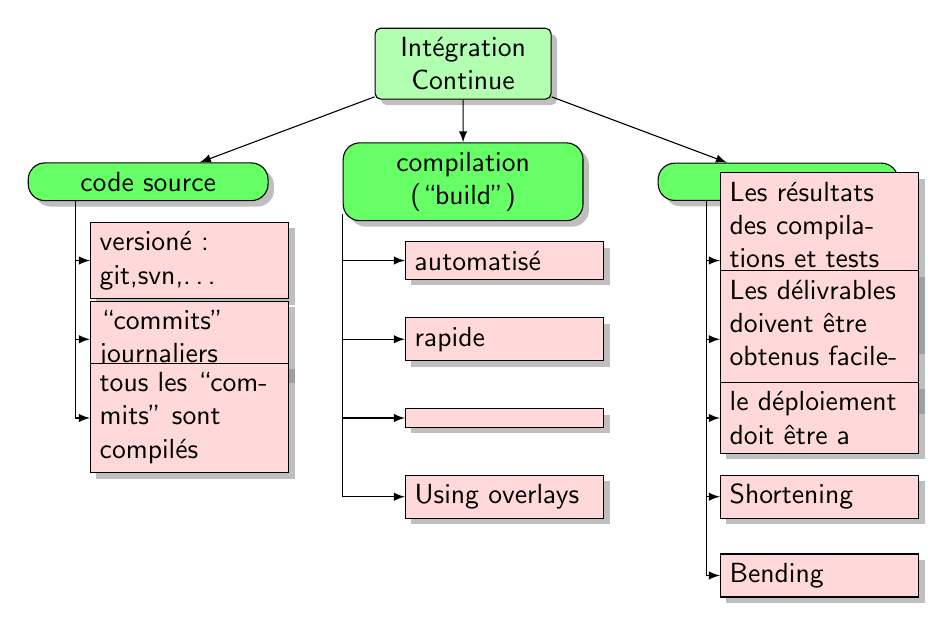
\begin{tikzpicture}[
  level 1/.style={sibling distance=40mm},
  edge from parent/.style={->,draw},
  >=latex]

% root of the the initial tree, level 1
\node[root] {Intégration Continue}
% The first level, as children of the initial tree
  child {node[level 2] (c1) {code source}}
  child {node[level 2] (c2) {compilation (``build'')}}
  child {node[level 2] (c3) {sorties}};

% The second level, relatively positioned nodes
\begin{scope}[every node/.style={level 3}]
\node [below of = c1, xshift=15pt] (c11) {versioné : git,svn,\dots};
\node [below of = c11] (c12) {``commits'' journaliers};
\node [below of = c12] (c13) {tous les ``commits'' sont compilés};

\node [below of = c2, xshift=15pt] (c21) {automatisé};
\node [below of = c21] (c22) {rapide};
\node [below of = c22] (c23) {};
\node [below of = c23] (c24) {Using overlays};

\node [below of = c3, xshift=15pt] (c31) {Les résultats des compilations et tests doivent être partagés};
\node [below of = c31] (c32) {Les délivrables doivent être obtenus facilement};
\node [below of = c32] (c33) {le déploiement doit être a};
\node [below of = c33] (c34) {Shortening};
\node [below of = c34] (c35) {Bending};
\end{scope}

% lines from each level 1 node to every one of its "children"
\foreach \value in {1,2,3}
  \draw[->] (c1.195) |- (c1\value.west);

\foreach \value in {1,...,4}
  \draw[->] (c2.195) |- (c2\value.west);

\foreach \value in {1,...,5}
  \draw[->] (c3.195) |- (c3\value.west);
    % \node [draw,rectangle,fill=gray] at (8,0) {Intégration continue}
    % child {node [draw,rectangle,fill=gray] {compilations automatiques}}
    % child {node [draw,rectangle,fill=gray] {tests automatiques}}
    % child {node [draw,rectangle,fill=gray] {``commits'' journaliers}}
    % child {node [draw,rectangle,fill=gray] {tous les ``commits'' doivent être compilés et testés}}
    % child {node [draw,rectangle,fill=gray] {la compilation doit rester rapide}}
    % child {node [draw,rectangle,fill=gray] {le test ne doit pas se faire dans l'environnement de production}}
    % child {node [draw,rectangle,fill=gray] {les résultats des dernières compilations et tests doivent être visibles}}
    % child {node [draw,rectangle,fill=gray] {le déploiement doit être automatisé}};

  
   % \node[draw,rectangle,color=black] {Intégration continue}
   % node[] {dépôt du code source \textbf{versionné}}
   % child { node[] {compilations automatiques} }
   % child { node[] {tests automatiques} }
   % child { node[] {``commits'' journaliers} }
   % child { node[] {tous les ``commits'' doivent être compilés} }
   % child { node[] {la compilation doit rester rapide} }
   %    child { node[] {le test ne doit pas se faire dans l'environnement de production} }
   %    child { node[] {le dernier délivrable doit être disponible facilement} }
   %    child { node[] {les résultats des dernières compilations et tests doivent être visibles} }
   %    child { node[] {le déploiement doit être automatisé} }
   %  } ;
  \end{tikzpicture}
    
\end{frame}



% L'intégration continue à Inria
% ******************************
\inriaswitchcolors{blue}
\section{L'intégration continue à l'Inria}

\begin{frame}{https://ci.inria.fr/}
\begin{tikzpicture}
  \node[] (root) {};
  \node[below=3.5cm of root] (root_south) {};
  \node[] (cimain)  {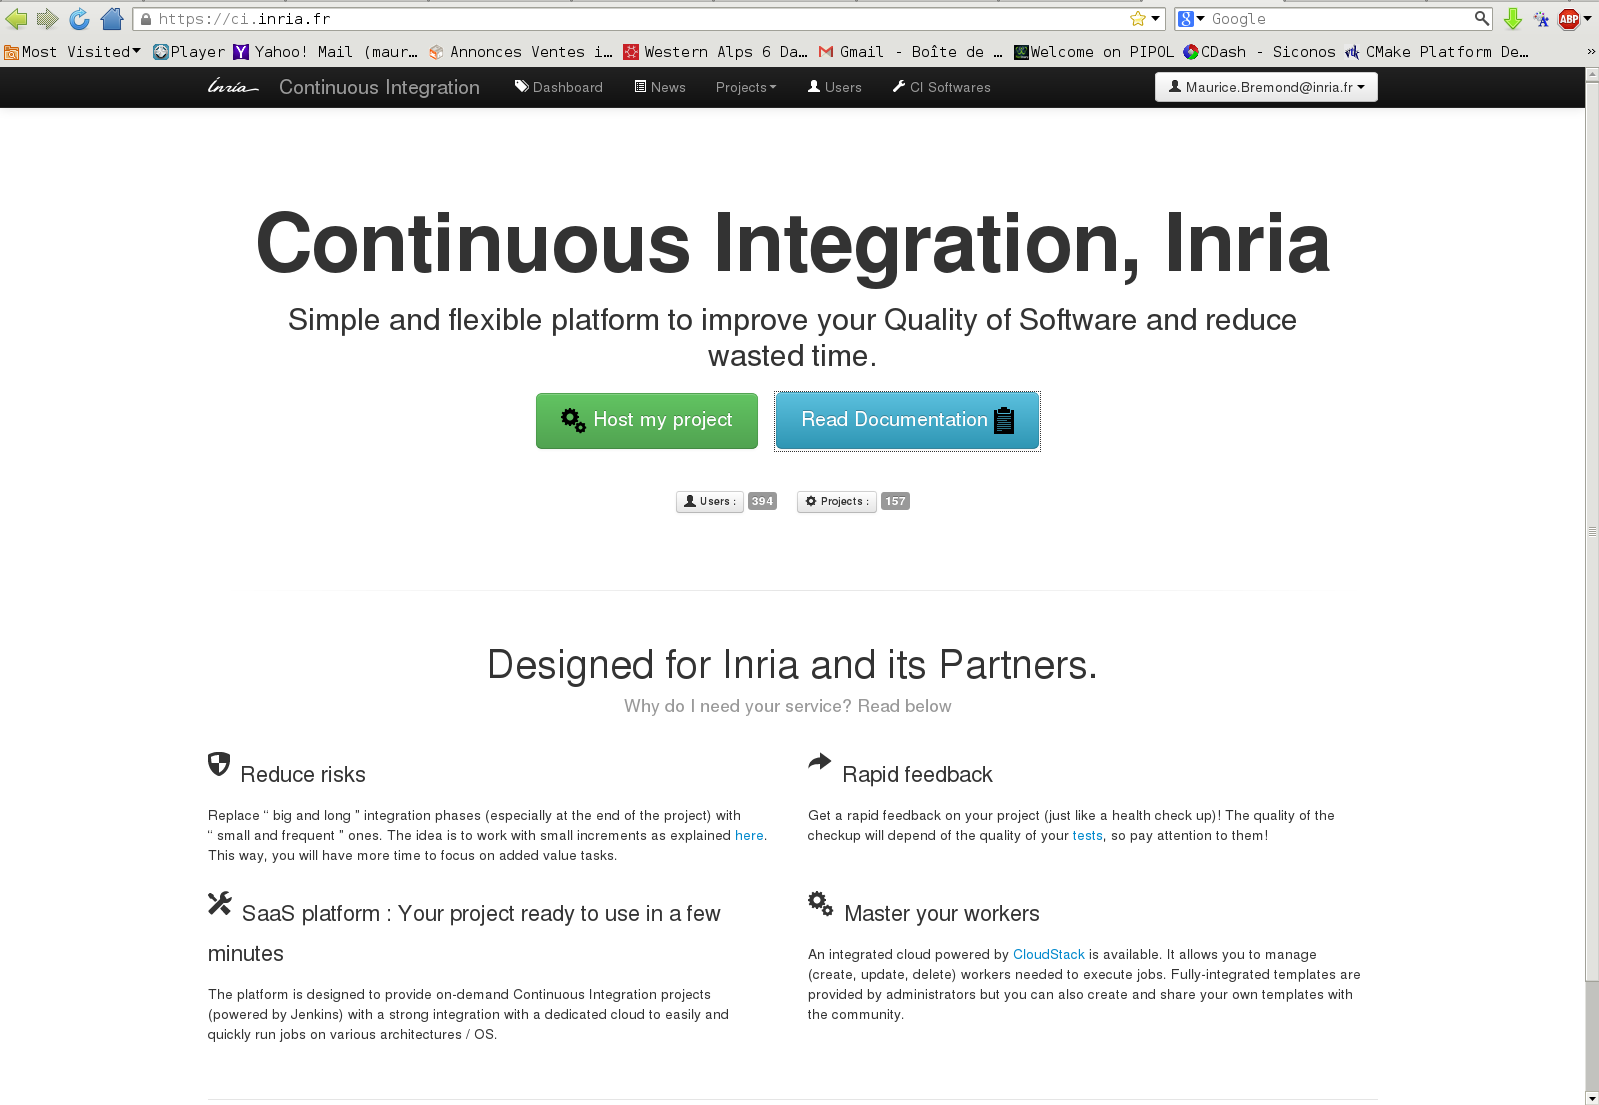
\includegraphics[width=.9\textwidth] {images/cimain.png}};
  \node[right=1.1cm of root_south] (cidoc)  {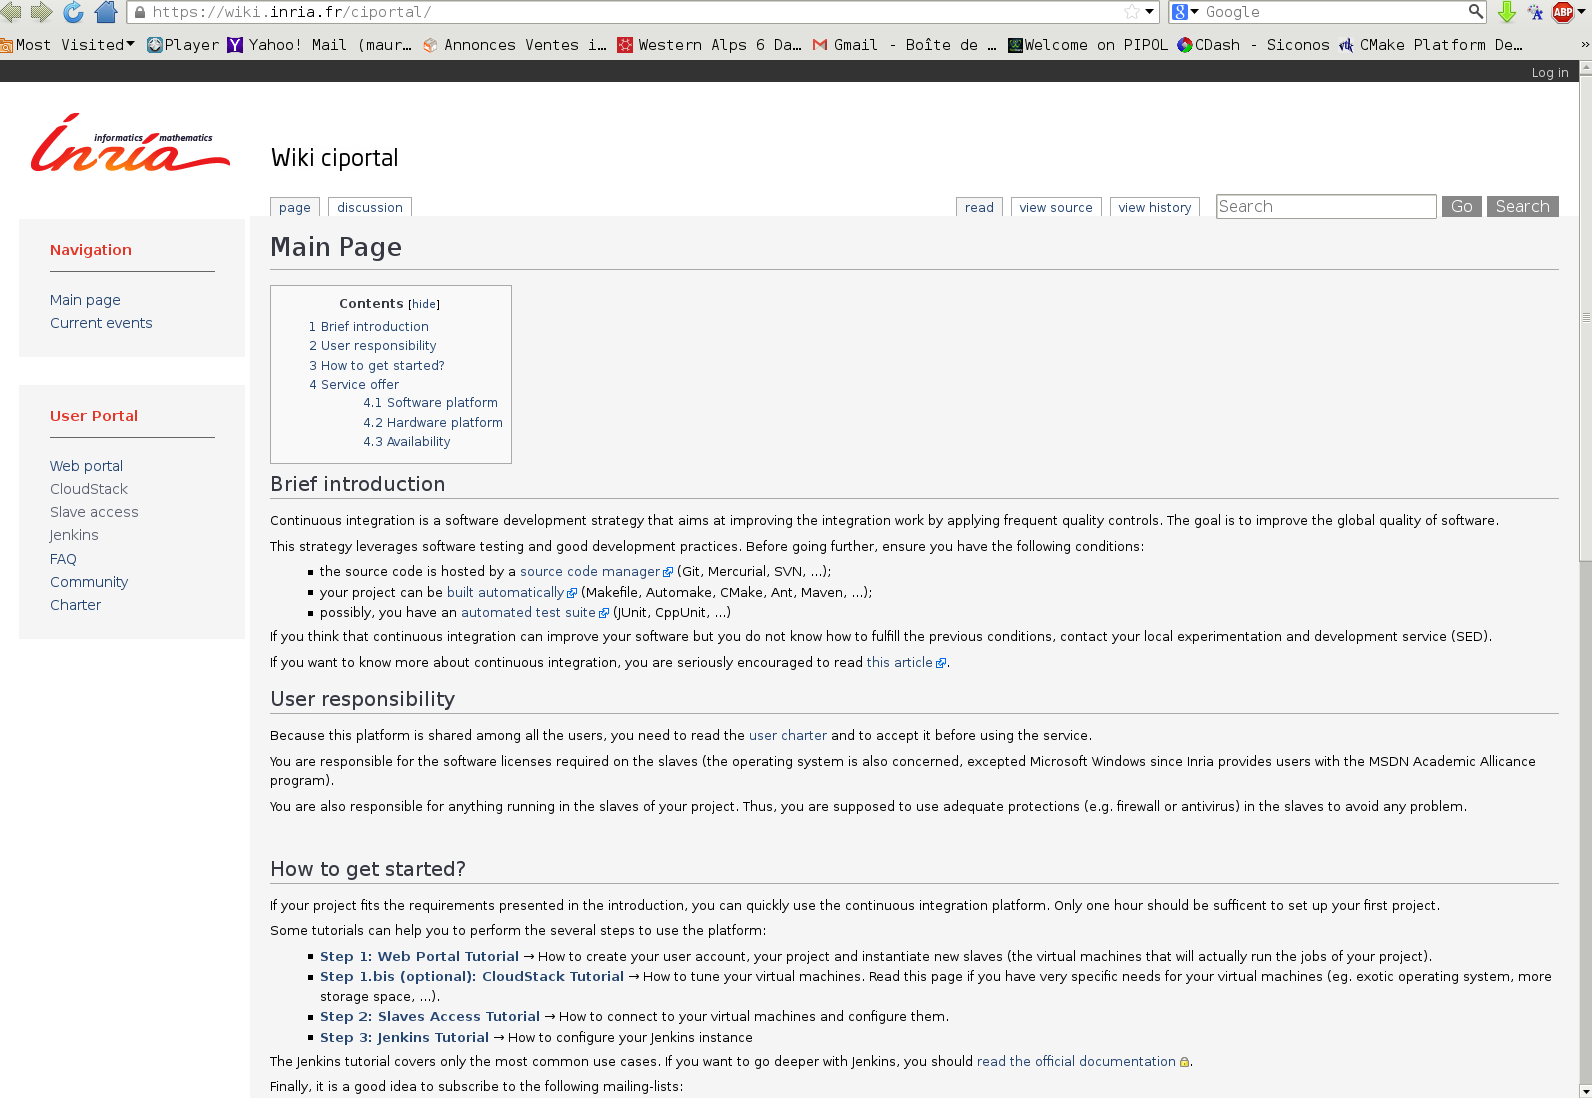
\includegraphics[width=.9\textwidth] {images/cidoc.png}};
  \node[draw,ellipse,minimum height=.8cm,minimum width=2.5cm,thick,color=red] at (.7,0.8) (ok) {};
  \path[->, thick, color=red] (.6,.2) edge [bend right] (.9,-.2);
\end{tikzpicture}
\end{frame}

\begin{frame}
\end{frame}



% Retour d'expérience
% *******************
\inriaswitchcolors{green}
\section{Un retour d'expérience}
\frame{\tableofcontents[currentsection]}

\subsection{Contexte de développement}
\tocsubsection

\subsubsection{Plateforme de réseau de capteurs: FIT IOT-LAB}
\begin{frame}{\subsubsecname} %{\subsecname}
  \setbeamercovered{transparent}
  \begin{itemize}
    \item <2->{Plateforme de réservation et expérimentation pour matériel réseau sans fil}
    \item <2->{Utilisé par des chercheurs depuis leur bureau}
    \item <2->{Déploiement à large échelle, 3000 nœuds capteurs}
    \item <2->{Projet d'une durée de 10ans}
  \end{itemize}
  \onslide <3-> ~\\~\\ Réservation, configuration et mise à disposition de nœuds capteurs.
\end{frame}


\begin{frame}{\subsubsecname} %{\subsecname}

  IMAGE DE LA PLATEFORME COMPLETE

\end{frame}

\subsubsection{Contexte de l'application}
\begin{frame}{\subsubsecname} %{\subsecname}
  \begin{itemize}
    \item Application mise en production
    \item Exécution sur une carte ARM avec Linux embarqué (perf...)
    \item Commande par interface REST (web)
    \item Interaction par port série avec un OS temps réel sur un micro-contrôleur
    \item multithread, multiprocess
    \item Il faut préserver les interfaces à tout moment
  \end{itemize}
\end{frame}


\subsubsection{Pourquoi avoir mis place de l'intégration continue}
\begin{frame}{\subsubsecname} %{\subsecname}
  \begin{itemize}
    \item Une pratique qui m'intéresse
    \item Logiciel final doit être fiable
    \item Source d'erreurs aléatoires
    \item Déployé à large échelle
  \end{itemize}
\end{frame}



\subsection{Outils mis en place}
\tocsubsection

\subsubsection{Présentation des outils}
\begin{frame}{Outils mis en place}

  Gestionnaire de versions: \texttt{git} \\ ~ \\

  \begin{tabular}{ l | l l | p{3.5cm} }
    Language         & \texttt{Python}     & \texttt{C}    & Utilisation dans Jenkins \\ \hline
    Script de build  & \texttt{setuptools} & \texttt{Make} & Bash~shell, \texttt{EnvInject} \texttt{virtualenv}\\
    Compilation      & ~                   & \texttt{gcc}  & ~ \\
    Tests            & \texttt{unittest}, \texttt{mock}, \texttt{nose}
                     & \texttt{gtest} \texttt{(C++)}
                     & Junit, Chuck Norris\\
    Couverture       & \texttt{nose-xcover}
                     & \texttt{gcov}, \texttt{gcovr}
                     & Cobertura \\
   Qualité de code  & \texttt{pylint}, \texttt{pep8} & ~  & Violations \\
    ~ & ~  & ~ & \\
    Lignes de code   &  $3000$        &  $1500$  &  $0$  \\
    Lignes de tests  &  $1600 + 400$  &  $1300$  &  $0$  \\
% 1600 tests U + 400 tests intégration
    Lignes de build  &  $300$         &  $170$   &  $50$ \\

% (SQLite 3.8 == 1084 * plus de tests que de code 84k source (hors blank et commentaires))
  \end{tabular}
\end{frame}


\subsubsection{Jenkins}
\begin{frame}{Présentation outils}{Jenkins}
  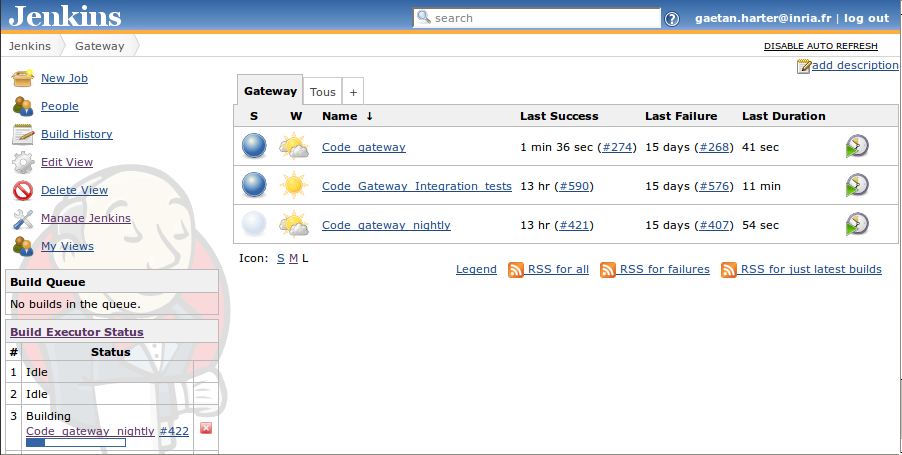
\includegraphics[width=\linewidth]{images/jenkins}
\end{frame}

\begin{frame}{Configuration d'un build}{Jenkins}
  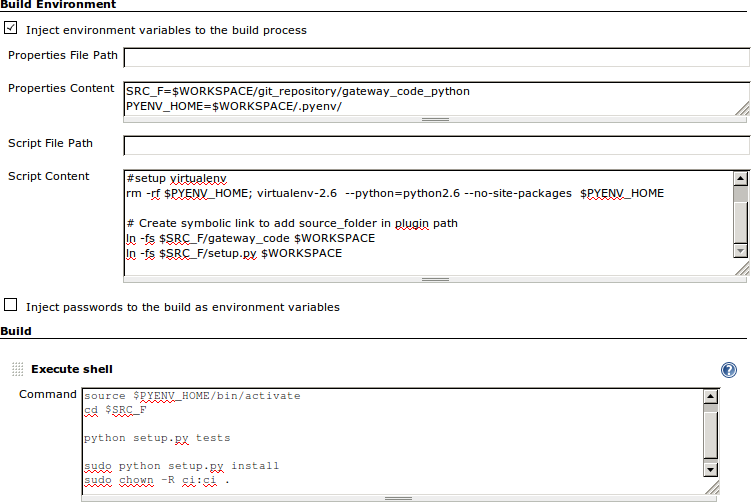
\includegraphics[width=\linewidth]{images/build_configuration}
\end{frame}


\begin{frame}{Cobertura}{Jenkins}
        % Pour moi, l'outil le plus important (après Chuck Norris forcément)
  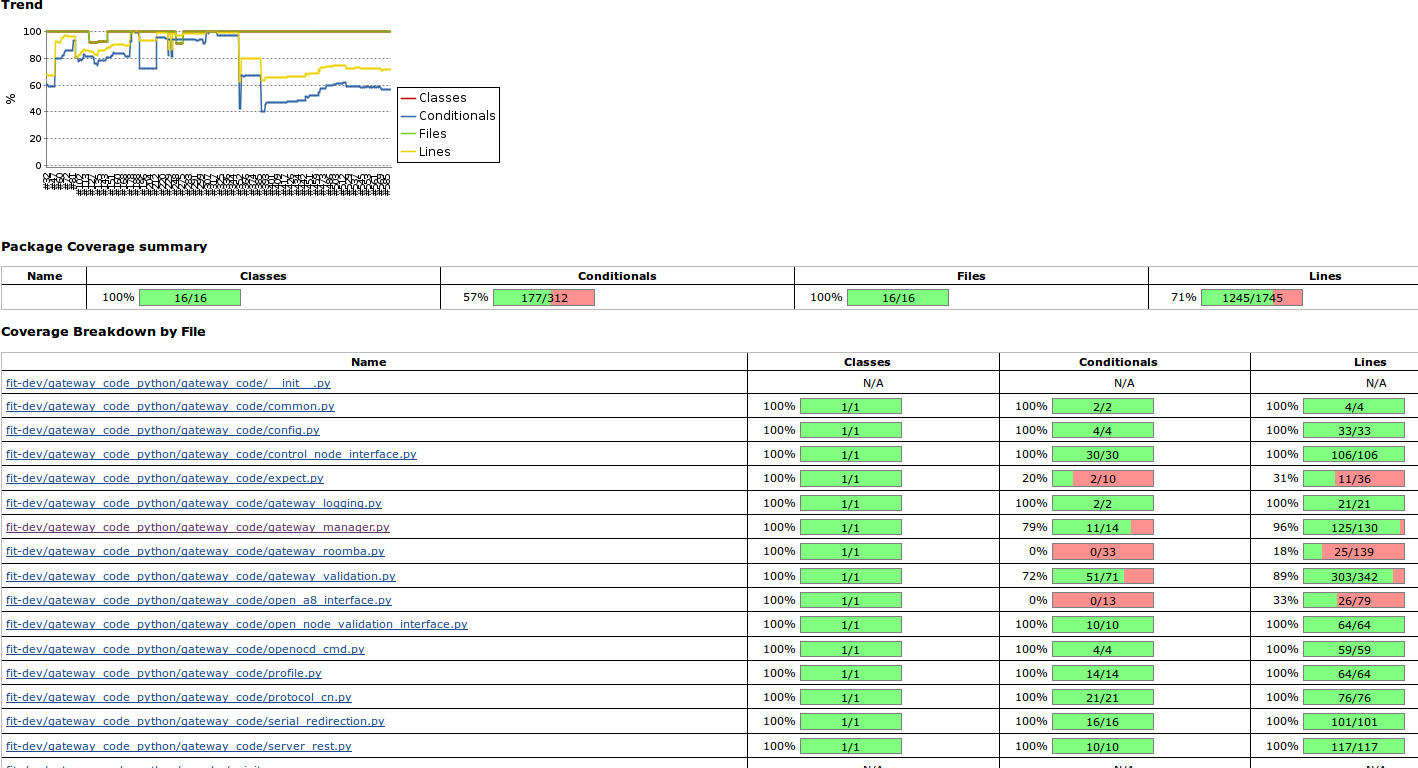
\includegraphics[width=\linewidth]{images/cobertura}\\
\end{frame}
\begin{frame}{Junit - Violations}{Jenkins}
  \begin{center}
        % Juste pour montrer
    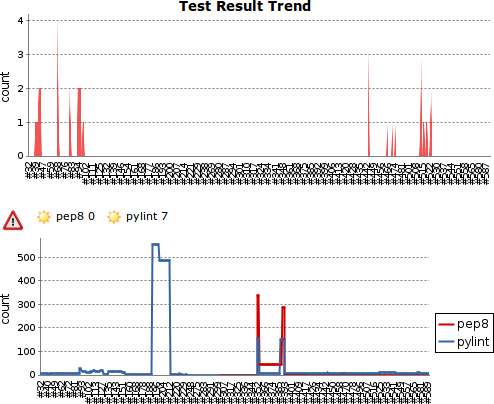
\includegraphics[height=0.8\textheight]{images/junit_violations}\\
  \end{center}
\end{frame}
\begin{frame}{Chuck Norris}{Jenkins}
  % Le plus important des plugins
  \begin{center}
    \begin{tabular}{ l |l }
      Build KO & Build OK \\ \hline
        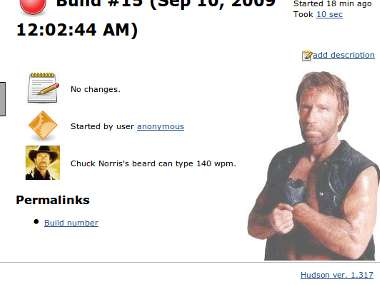
\includegraphics[height=4cm]{images/chuck_full} &
      
\includegraphics[height=4cm]{images/chuck_happy}
        %
\includegraphics[height=4cm]{images/chuck_angry}
      \\
    \end{tabular}
  \end{center}
  Chuck Norris Facts:
  \begin{itemize}
    \item Chuck Norris can unit test an entire application with a single assert.
    \item Chuck Norris can divide by zero.
    \item ...
  \end{itemize}
\end{frame}




\subsection{Bilan}
\tocsubsection


\subsubsection{Développement logiciel}
\begin{frame}{\subsubsecname}{\subsecname}
  \setbeamercovered{transparent}

  \begin{itemize}
    \item <2-> Mise en place d'un script de \texttt{build}
      \begin{itemize}
        \item Mise en place d'une procédure de test (pouvoir écrire et lancer un test)
        \item Procédure simple et conditionnée dans un script
      % \item Adhérence aux conventions d'architecture du language
      \end{itemize}
    \item <3->Tests nombreux et lancés en continue
      \begin{itemize}
        \item Apparition et gestion des cas d'erreurs (cas 'rares')
        \item Détection de problèmes tot (performance, permissions)
        \item Simplification de l'implémentation pour la testabilité
        \item Ajout au fur et à mesure des fonctionnalités (non régression)
      % \item Suivi des bugs
      \end{itemize}
    \item <4-> Couverture de code
      \begin{itemize}
        \item Même si $<100\%$, savoir ce qui est 'validé' et ce qui ne l'est pas
      \end{itemize}
    \item <5-> Qualité de code (Python)
      \begin{itemize}
        \item Remplace la phase de compilation (vérification syntaxique)
        \item Détection statique d'erreurs
        \item Standardisation de la mise en forme, lisibilité (PEP8)
      \end{itemize}
  \end{itemize}
  \onslide <6-> Maîtrise et confiance dans le logiciel développé
\end{frame}

\subsubsection{Personnel}
\begin{frame}{\subsubsecname}{\subsecname}
  \begin{itemize}
    \item Découverte de beaucoup d'outils
    \item Confort dans le développement (non régression)
    \item Retours positifs après premières utilisations
  \end{itemize}
\end{frame}

\subsubsection{Voies d'amélioration}
\begin{frame}{\subsubsecname}{\subsecname}
  \begin{itemize}
    \item Passer les configurations Jenkins dans des scripts versionnés
    \item Grouper Python et C dans le build python
    \item Inclusion d'autres développeurs
    \item 100\% de couverture de code
  \end{itemize}
\end{frame}

\end{document}
